% for landscape posters, use "a4paper, landscape"
\documentclass[a4paper]{article}
\usepackage{better_poster}
\usepackage{graphicx}
\usepackage{caption}
\usepackage{multicol}


% ---- fill in from here
% poster size - this will scale the poster to the given size.
% for landscape posters add ", landscape" to the postersize command.
\postersize{a1paper}

% authors
\title{\textit{Resonant Landscapes}}
\author{Tate Carson \& Carter Gordon, Dakota State University, USA}

% type of poster: [exp]erimental results, [methods], [theory]
% Disclaimer: the original classification had "study" and "intervention" as separate categories. I group them under experimental results.
\newcommand\postertype{exp} % [exp],[methods],[theory]

\begin{document}

% main point of your study
\makefinding{
    \textit{\textbf{Resonant Landscapes}} creates a \textbf{hybrid place}, merging natural soundscapes with urban spaces through \textbf{ambisonic audio} and GPS technology.
}


% \makemain{
% }{

% }


% the main text of your poster goes here
\makemain{

    % you can have 1 or 2 columns
    \raggedcolumns
    \raggedright
    \small
    % \begin{multicols}{1}
    \section{Introduction}
    \begin{compactitem}
        \item Web-based app overlaying South Dakota state park soundscapes onto Dakota State University's campus
        \item Uses frugal innovation: existing smartphone sensors and open-source software
        \item 2nd-order ambisonic audio with GPS integration
        \item Body-oriented tracking and dynamic soundscapes based on user proximity
    \end{compactitem}

    \section{Significance}
    \begin{compactitem}
        \item Creates "hybrid place" of natural and urban soundscapes
        \item Promotes ecological awareness and attentive listening
    \end{compactitem}

    % \columnbreak

    \section{User Experience}
    \begin{compactitem}
        \item Interactive campus map with listening spots
        \item Audio playback within 15-meter radius; body-oriented tracking at epicenters
    \end{compactitem}

    \section{Technical Details}
    \begin{compactitem}
        \item Core Audio OctoMic
        \item Web tech: React, Tailwind CSS, Resonance Audio SDK
        \item Smartphone sensors: GPS, gyroscope, accelerometer
    \end{compactitem}

    \section{Future Work}
    \begin{compactitem}
        \item Enhance user experience through iterative design
        \item Expand soundscape database for diverse ecosystems
        \item Longer audio playback
    \end{compactitem}
    % \end{multicols}
}
% If you have extra figures or data to show
\makeextracolumn{

    \begin{center}
        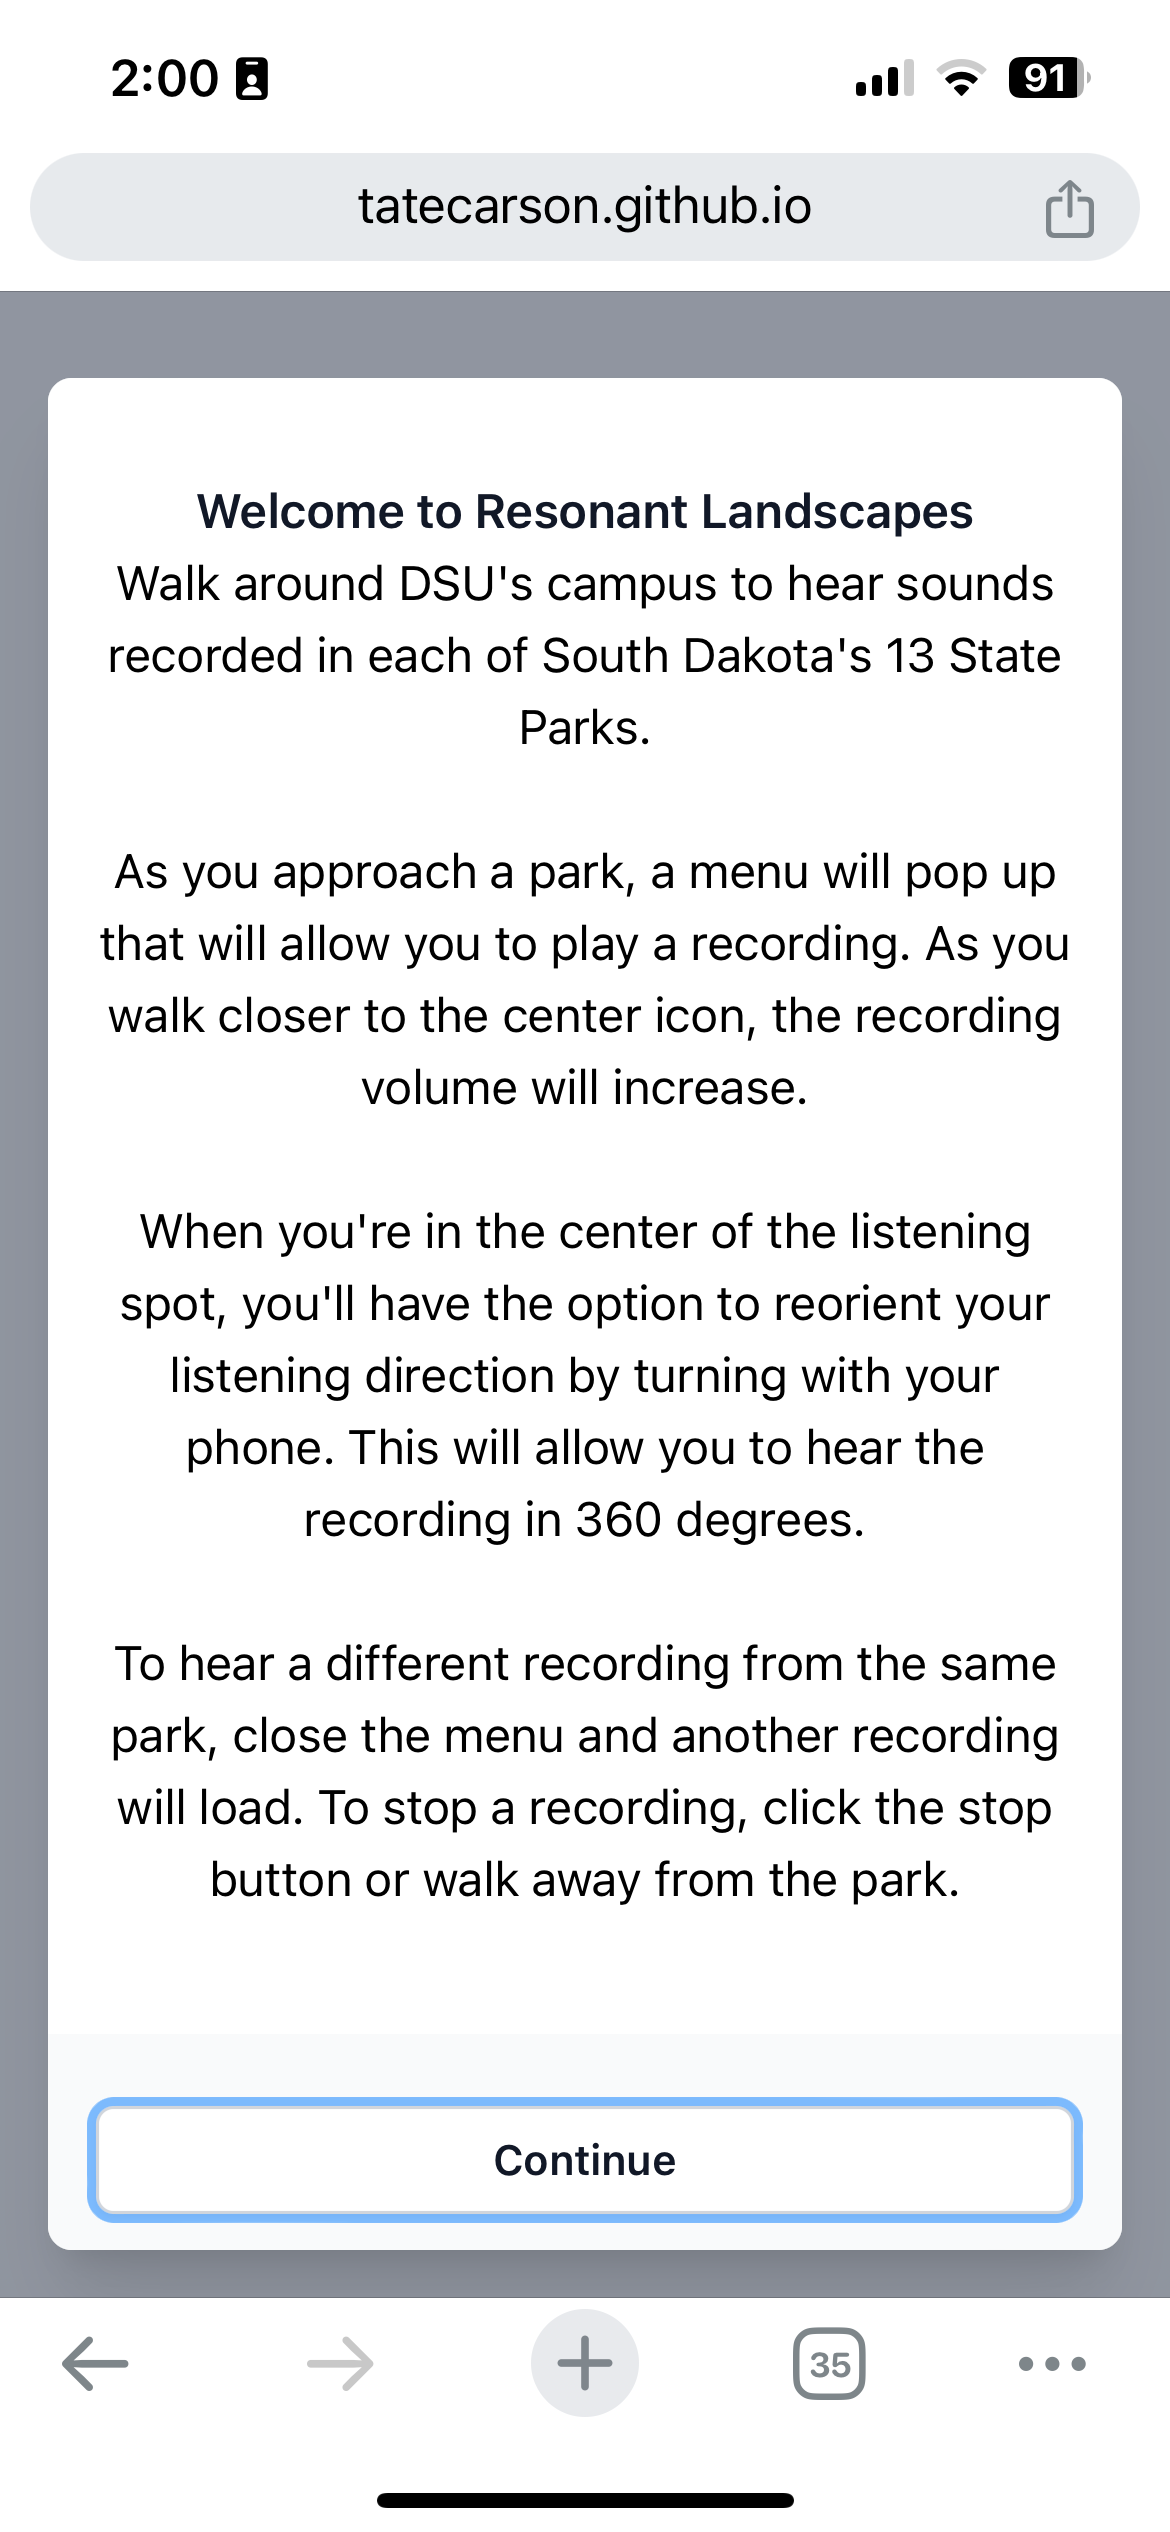
\includegraphics[width=0.44\linewidth]{figures/intro.PNG}
        \vspace{1cm}
        \hspace{0.5cm}
        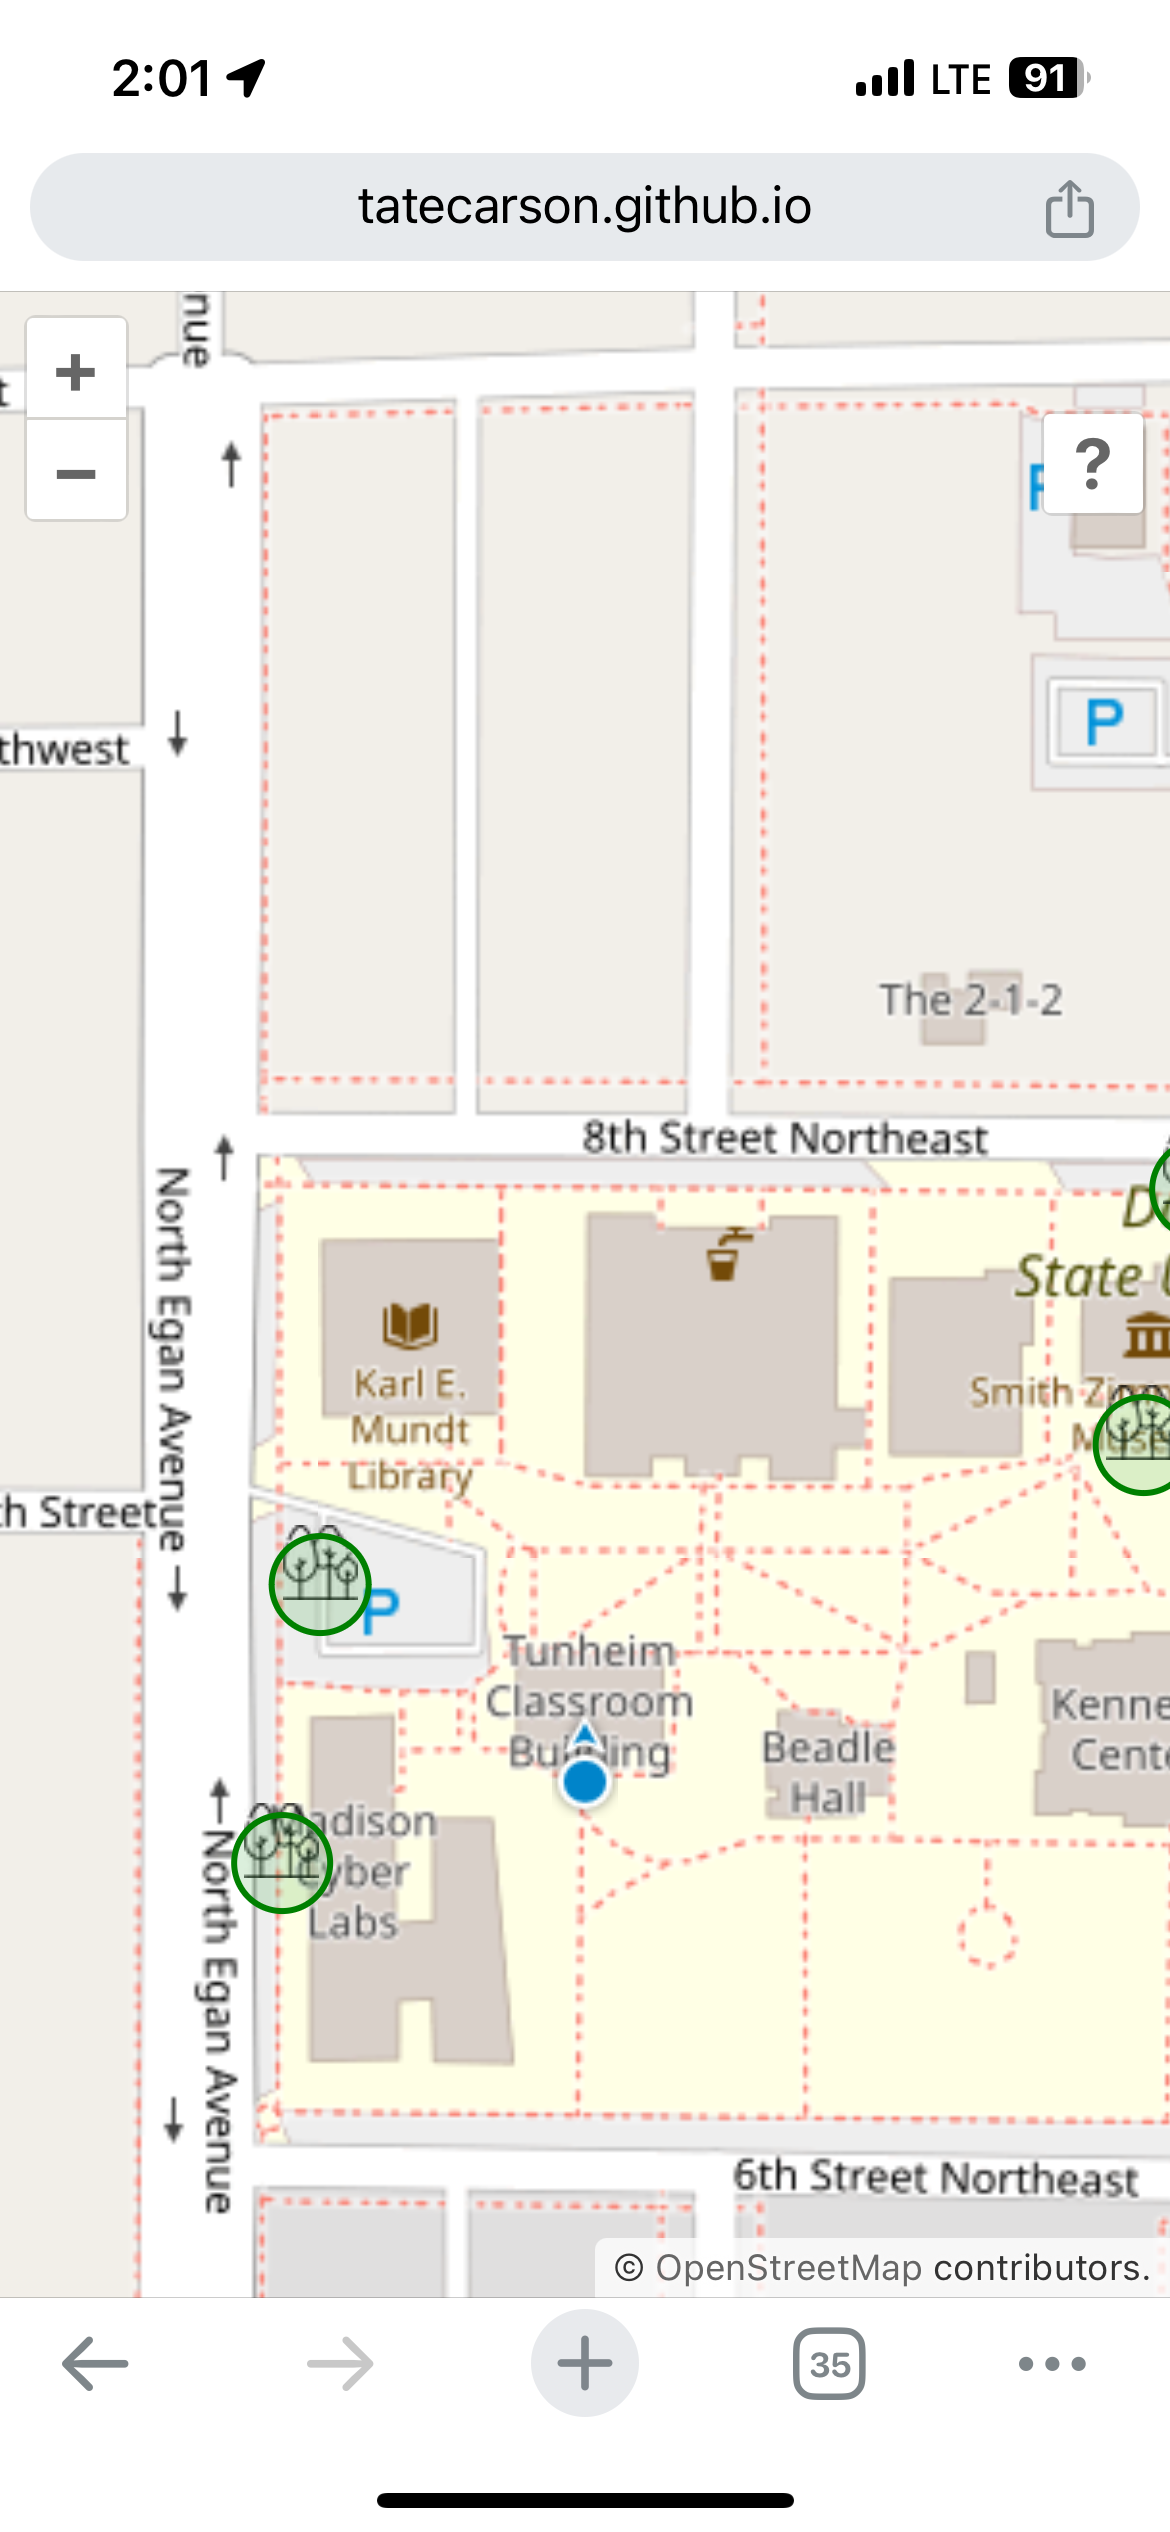
\includegraphics[width=0.44\linewidth]{figures/overview.PNG}
        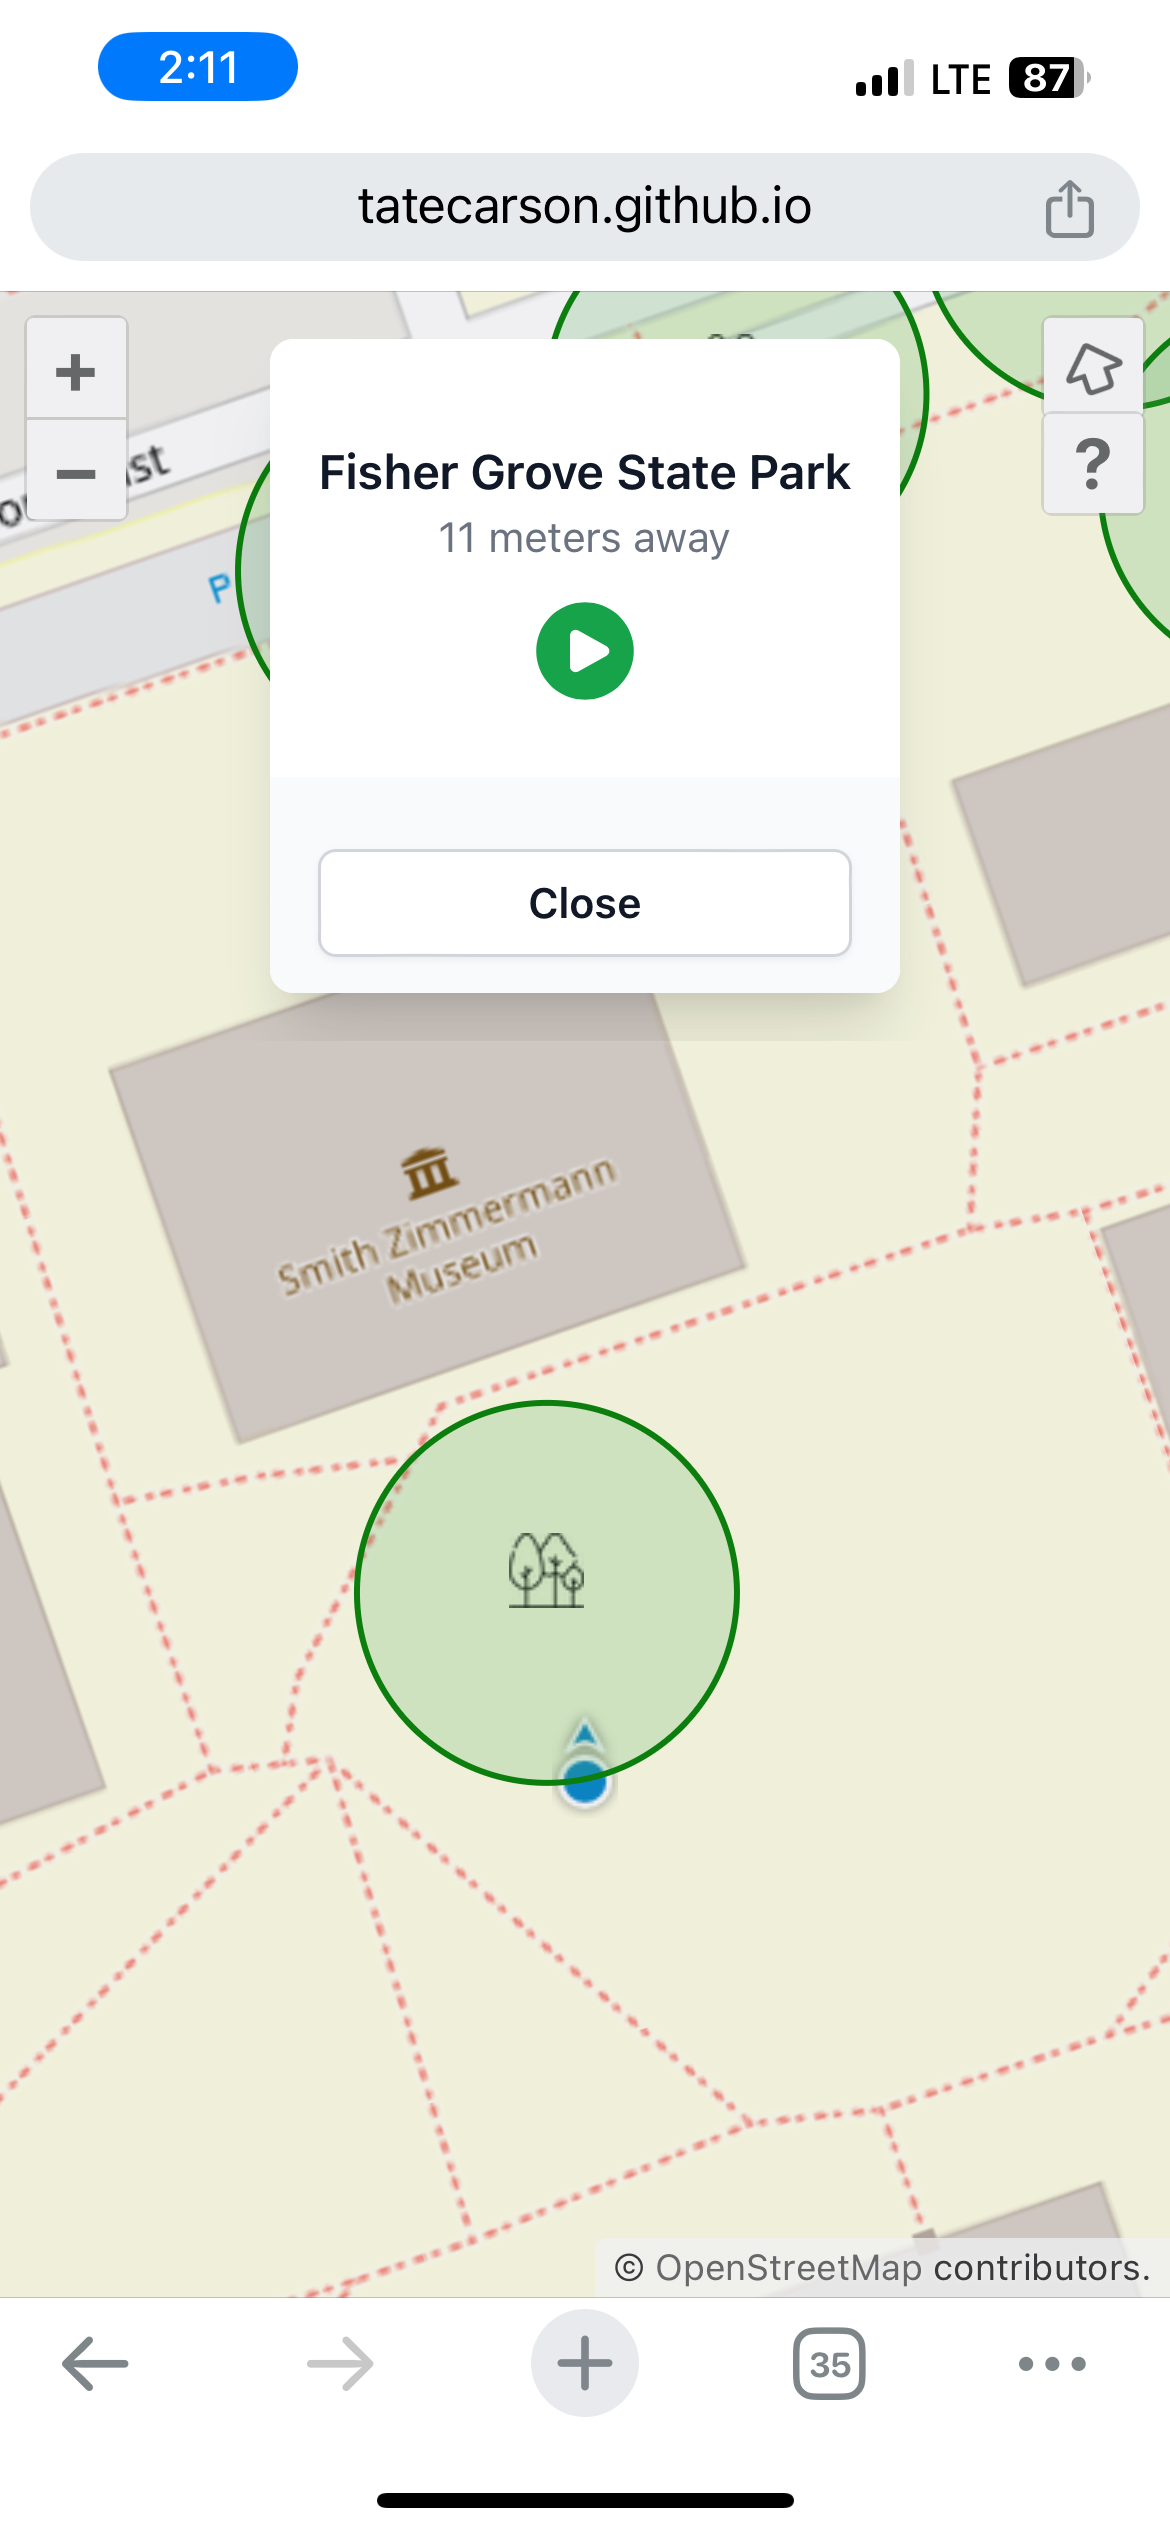
\includegraphics[width=0.44\linewidth]{figures/fisher-grove-11-meters.png}
        \hspace{0.5cm}
        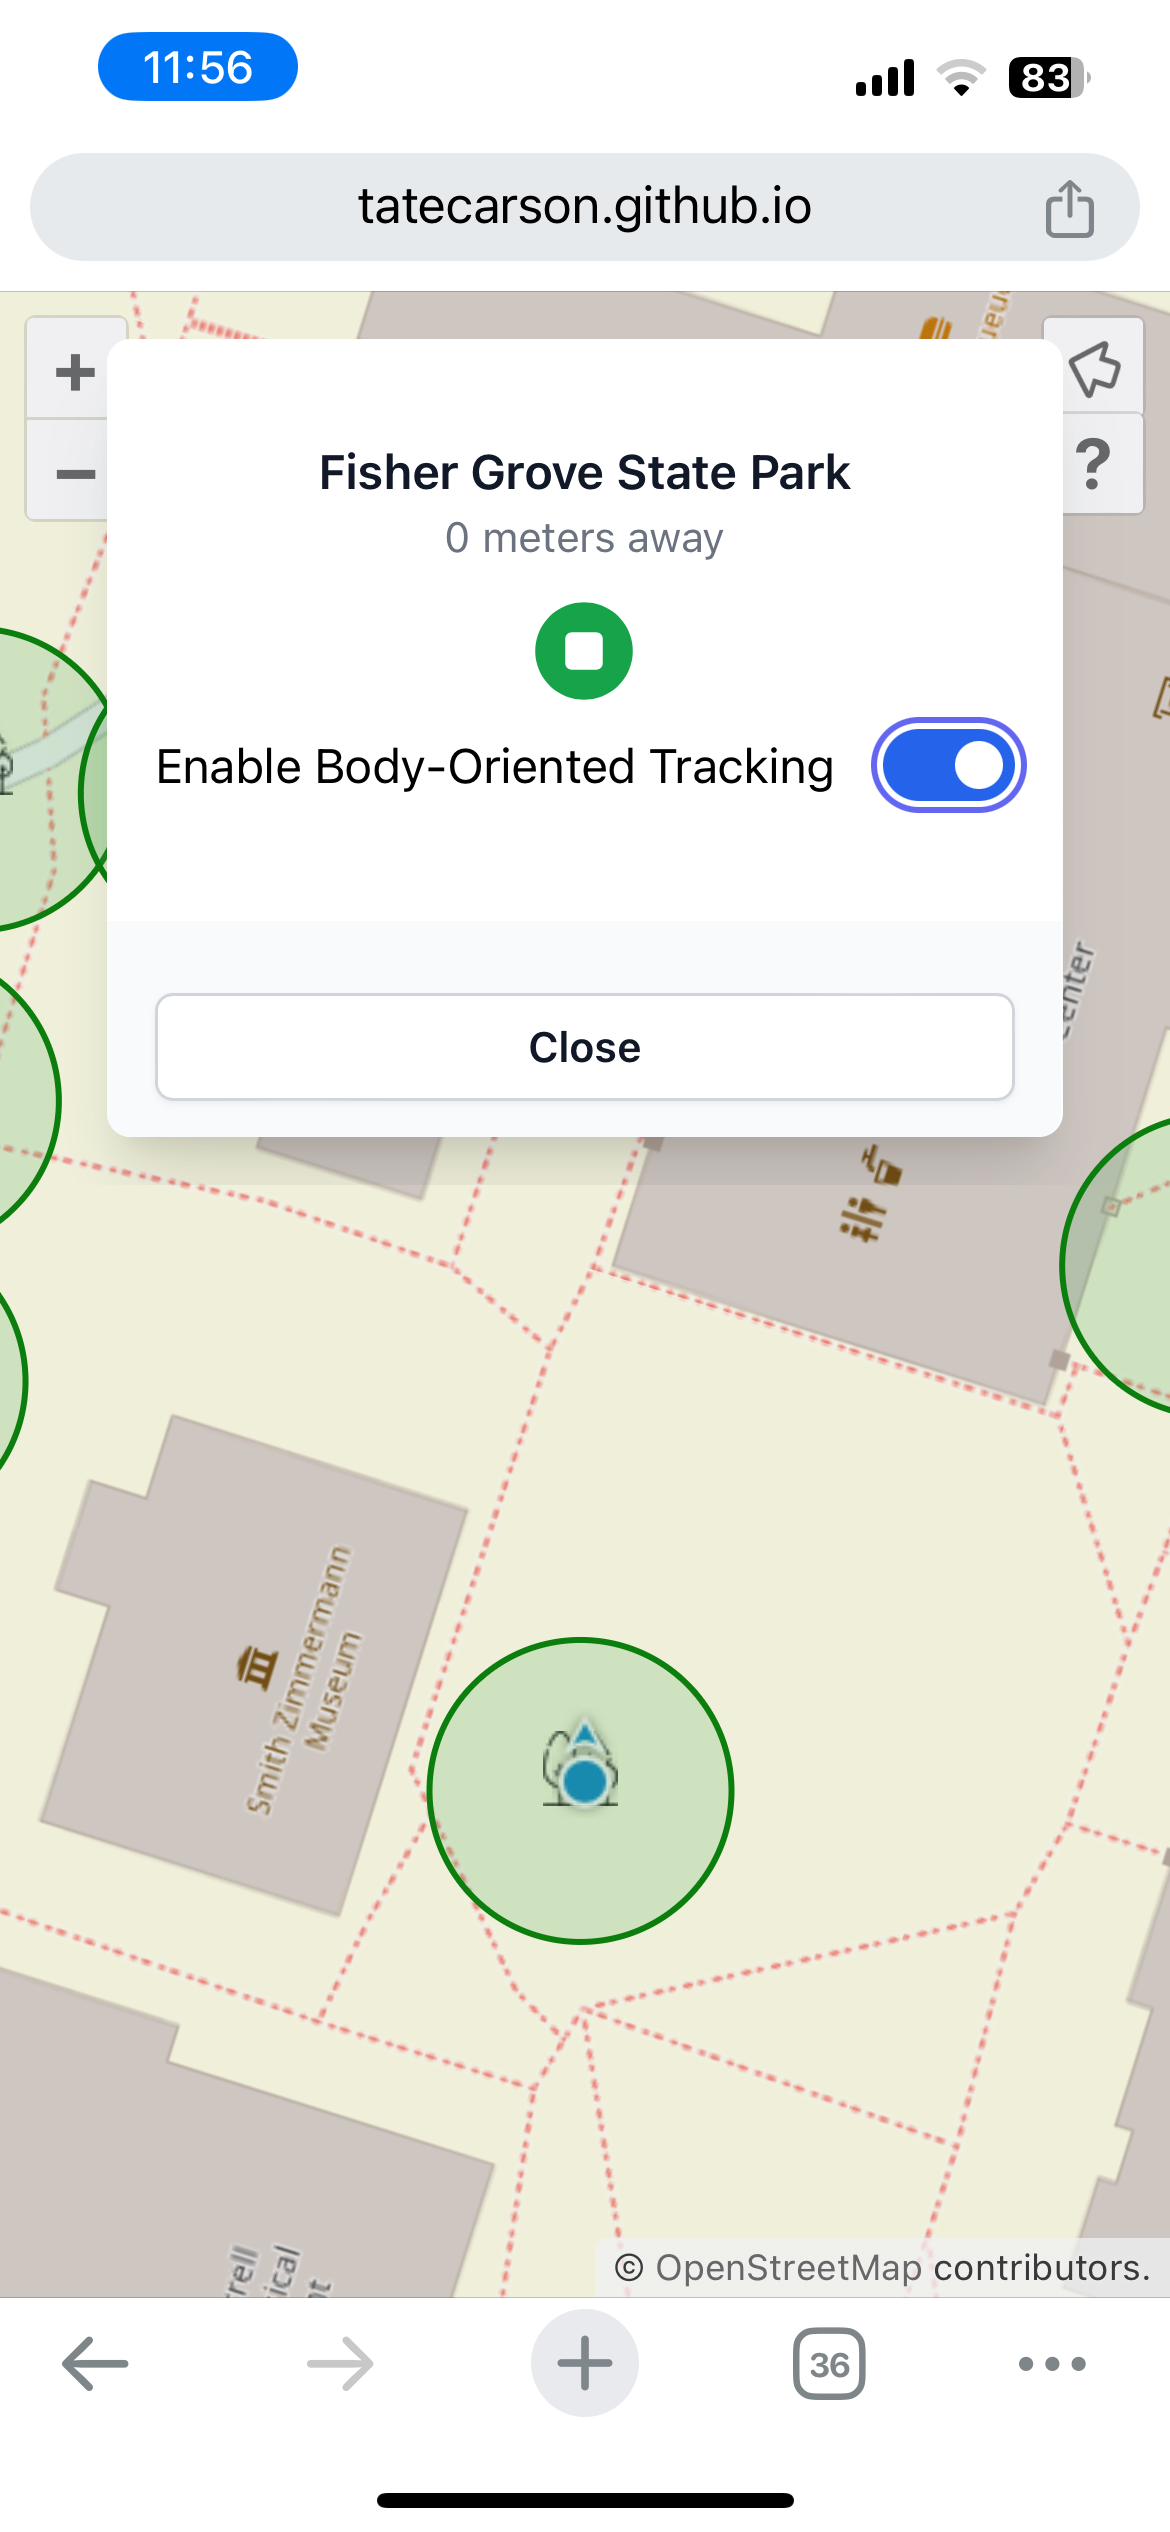
\includegraphics[width=0.44\linewidth]{figures/IMG_0424.PNG}


    \end{center}


}


% footer
% generate qr code from https://www.qr-code-generator.com/ and replace qr_code.png
% default: barcode on the left
\makealtfooter{images/DSU_UniversityLogo_Stacked_BLK.png}{images/qr-code.png}

% replace with this like for barcode on the right
%\makealtfooter{images/uni_logo.png}{images/qr-code.png}

\end{document}